\documentclass[10pt,a4paper]{article}
\usepackage{amsmath,amssymb,amsfonts,amsthm}
\usepackage{graphicx}
\usepackage[margin=1in]{geometry}
\usepackage{hyperref}
\usepackage{titling}
\usepackage{mathpazo} % Palatino font
\usepackage{microtype}
\usepackage{url}
\usepackage{parskip} %removes indentation and spacing between paras
\usepackage{enumitem}

%for state diagrams
\usepackage{tikz}
\usepackage{booktabs} % nicer table rules with built-in spacing
\usetikzlibrary{automata, positioning, arrows.meta}

% Remove vertical space between list items globally
\setlist{nosep}

% Define theorem-like environments
\theoremstyle{definition} % 'definition' style keeps text upright (not italic) which is easier to read for reports
\newtheorem{statement}{Statement}

%text rendering for pipe symbol
\usepackage[T1]{fontenc}

% include code
\usepackage{listings}
% Optional: style for Verilog syntax highlighting
\lstdefinestyle{verilog}{
    language=Verilog,
    basicstyle=\ttfamily\footnotesize,
    keywordstyle=\bfseries\color{blue},
    commentstyle=\color{gray},
    numbers=left,
    numberstyle=\tiny,
    frame=single,
    breaklines=true
}

% colours for listings (tikz loads xcolor, but be explicit)
\usepackage{xcolor}

\hypersetup{
    colorlinks=true,
    linkcolor=blue,
    citecolor=blue,
    urlcolor=blue
}
% bring title up
\setlength{\droptitle}{-6em}

\usepackage{titlesec}
\titlespacing*{\section}{0pt}{0.5em}{4pt}

%----------------------------------------------------------------------------------------
%   TITLE SECTION
%----------------------------------------------------------------------------------------

\title{3B2 FPGA Programming Lab Report}

% Authors are listed in a comma-separated list with superscript numbers indicating affiliations
\author{%
	Liu Zihe\textsuperscript{1}\thanks{CRSID: zl559. Date: 20th February 2026}
}

% Affiliations are output in the \date{} command
\date{\footnotesize\textsuperscript{\textbf{1}}University of Cambridge}

\begin{document}

\maketitle

\begin{abstract}
    \noindent This report documents the design, implementation and testing of a traffic light controller on an Altera Cyclone V FPGA. A three-state finite state machine controlling a pedestrian crossing is described in Verilog, compiled, and configured onto a DE1-SoC board via JTAG, and is improved with a vehicle lockout.
\end{abstract}

%========================================================================================
% SECTION: TLC Design
%========================================================================================
\section{Traffic Light Controller Design}

We design a controller for a pedestrian light-controlled crossing, satisfying the following requirements:
\textit{
    \begin{enumerate}
        \item The initial state is vehicle GREEN and pedestrian RED.
        \item State changes occur only on demand: a pedestrian request or a reset.
        \item After a request, the sequence is: vehicle YELLOW for 5\,s, then vehicle RED with pedestrian GREEN for 10\,s, then back to the initial state.
        \item An asynchronous reset returns to the initial state from any state.
    \end{enumerate}
}

These requirements are captured by a three-state FSM shown in Figure~\ref{fig:state-diagram}. State \texttt{G} is the idle state with vehicle GREEN and pedestrian RED. A pedestrian \texttt{request} triggers a transition to state \texttt{Y} (vehicle YELLOW), which serves as a warning to vehicles. After a 5\,s timeout the FSM enters state \texttt{R} (vehicle RED, pedestrian GREEN), allowing pedestrians to cross. A 10\,s timeout then returns the FSM to state \texttt{G}. An asynchronous active-low \texttt{reset} forces the FSM back to state \texttt{G} from any state.

% State diagram (tikz figure from external file)
% ============================================================
% TLC State Diagram — paste into your report
% Requires: \usepackage{tikz}
%           \usetikzlibrary{automata, positioning, arrows.meta}
% ============================================================
\begin{figure}[htbp]
    \centering
    \begin{tikzpicture}[->, >=Stealth, shorten >=1pt, auto, node distance=4.5cm,
            semithick, every state/.style={minimum size=1.8cm, font=\large}]

        % --- States ---
        \node[state, fill=green!15]   (G) {$\mathbf{G}$};
        \node[state, fill=yellow!25]  (Y) [right of=G] {$\mathbf{Y}$};
        \node[state, fill=red!15]     (R) [right of=Y] {$\mathbf{R}$};

        % --- Transitions ---
        \path (G) edge [bend left=25]  node {\texttt{request}} (Y)
        (Y) edge [bend left=25]  node {5\,s timeout}     (R);
        \draw[->] (R.south west) .. controls +(0,-1.5) and +(0,-1.5) ..
        node[below, pos=0.5] {10\,s timeout} (G.south east);

        % --- Output labels ---
        \node[below=1.8cm of G, align=center, font=\footnotesize] {
            \underline{State G}\\[2pt]
            Veh: \textcolor{green!60!black}{\textbf{GREEN}}\\[2pt]
            Ped: \textcolor{red}{\textbf{RED}}\\[2pt]
            \texttt{output = 10001}
        };
        \node[below=1.8cm of Y, align=center, font=\footnotesize] {
            \underline{State Y}\\[2pt]
            Veh: \textcolor{yellow!70!black}{\textbf{YELLOW}}\\[2pt]
            Ped: \textcolor{red}{\textbf{RED}}\\[2pt]
            \texttt{output = 01001}
        };
        \node[below=1.8cm of R, align=center, font=\footnotesize] {
            \underline{State R}\\[2pt]
            Veh: \textcolor{red}{\textbf{RED}}\\[2pt]
            Ped: \textcolor{green!60!black}{\textbf{GREEN}}\\[2pt]
            \texttt{output = 00110}
        };

    \end{tikzpicture}
    \caption{State diagram for the traffic light controller FSM. The 5-bit output vector
        is \texttt{\{veh\_G, veh\_Y, veh\_R, ped\_G, ped\_R\}}. \texttt{reset} (active LOW, asynchronous) returns to state G from any state.}
    \label{fig:state-diagram}
\end{figure}

The outputs of each state and the transitions to the next states are summarised in Table~\ref{tab:state-table}. Each state activates exactly one vehicle light and one pedestrian light.

\begin{table}[htbp]
    \centering
    \caption{State table for the traffic light controller.}
    \label{tab:state-table}
    \begin{tabular}{c cccc ccccc}
        \toprule
                   & \multicolumn{4}{c}{Next State} & \multicolumn{5}{c}{Outputs}                                                                                                                     \\
        \cmidrule(lr){2-5} \cmidrule(lr){6-10}
        State      & \texttt{reset}                 & \texttt{request}            & 5\,s       & 10\,s      & \texttt{veh\_G} & \texttt{veh\_Y} & \texttt{veh\_R} & \texttt{ped\_G} & \texttt{ped\_R} \\
        \midrule
        \texttt{G} & \texttt{G}                     & \texttt{Y}                  & --         & --         & 1               & 0               & 0               & 0               & 1               \\
        \texttt{Y} & \texttt{G}                     & --                          & \texttt{R} & --         & 0               & 1               & 0               & 0               & 1               \\
        \texttt{R} & \texttt{G}                     & --                          & --         & \texttt{G} & 0               & 0               & 1               & 1               & 0               \\
        \bottomrule
    \end{tabular}
\end{table}

%========================================================================================
% SECTION: Verilog Implementation
%========================================================================================
\section{Verilog Implementation}

\lstinputlisting[style=verilog, caption={Basic traffic light controller.}, label={lst:tlc}]{tlc.v}

The Verilog code in Listing~\ref{lst:tlc} implements the FSM from Section~1. Key design choices made are:

\begin{itemize}
    \item \textbf{Clock division.} The DE1-SoC provides a 50\,MHz clock, but the TLC requires delays on the order of seconds. Rather than a separate clock divider module, a 29-bit counter (\texttt{count}) is used directly.
    \item \textbf{State encoding.} The three states are encoded with 2 bits (\texttt{G}=0, \texttt{Y}=1, \texttt{R}=2). A \texttt{default} case catches the unused encoding (3) and returns to state \texttt{G}.
    \item \textbf{Active-low inputs.} The DE1-SoC push-buttons output 0 when pressed. The reset is handled via \texttt{negedge reset} in the sensitivity list for asynchronous behaviour, and \texttt{request} is checked against \texttt{1'b0}.
    \item \textbf{Output mapping.} A combinational \texttt{always @(*)} block maps each state to a 5-bit output vector \texttt{[4:0]} = \texttt{\{veh\_G, veh\_Y, veh\_R, ped\_G, ped\_R\}}.
\end{itemize}

%========================================================================================
% SECTION: Compilation Results
%========================================================================================
\section{Compilation Results}

The design was compiled in Quartus Prime 25.1 Lite Edition targeting the Cyclone V 5CSEMA5F31C6 device. The full Compiler Flow Summary screenshot is in Appendix~\ref{sec:appendix}; key figures are in Table~\ref{tab:compilation}.

\begin{table}[htbp]
    \centering
    \caption{Compiler Flow Summary.}
    \label{tab:compilation}
    \begin{tabular}{lr}
        \toprule
        Resource                 & Count \\
        \midrule
        Logic utilisation (ALMs) & 27    \\
        Total registers          & 32    \\
        Total pins               & 8     \\
        \bottomrule
    \end{tabular}
\end{table}

The 32 registers break down as follows: the 2-bit \texttt{state} register, the 29-bit \texttt{count} register, and 1 synchroniser flip-flop for the \texttt{request} input. The 27 Adaptive Logic Modules (ALMs) house the counter increment, ad state transition logic. The 8 pins match the 3 inputs (\texttt{clk}, \texttt{request}, \texttt{reset}) and 5 outputs (\texttt{output[4:0]}).

%========================================================================================
% SECTION: Pin Assignment
%========================================================================================
\section{Pin Assignment}

During initial compilation, Quartus is free to assign design signals to any FPGA pin. However, the DE1-SoC board has hardwired connections between specific FPGA pins and on-board components (LEDs, push-buttons, clock oscillator), so pin assignments must be set manually via the Assignment Editor to match. The assignments used are shown in Table~\ref{tab:pins}. The design was recompiled after assigning pins so I/O is fitted correctly.

One limitation of the DE1-SoC is that all ten on-board user LEDs (LEDR0--LEDR9) are physically red. The traffic light colours (green, yellow, red) are therefore represented by LED position rather than colour: for example, LEDR8 represents vehicle GREEN even though the physical LED is red. Every output was placed at a different even integer position.

\begin{table}[htbp]
    \centering
    \caption{Pin assignments for the DE1-SoC board.}
    \label{tab:pins}
    \begin{tabular}{lll}
        \toprule
        Signal             & Pin                & Component          \\
        \midrule
        \texttt{clk}       & \texttt{PIN\_AF14} & 50\,MHz Clock      \\
        \texttt{request}   & \texttt{PIN\_AA15} & KEY1 (Push-button) \\
        \texttt{reset}     & \texttt{PIN\_AA14} & KEY0 (Push-button) \\
        \texttt{output[0]} & \texttt{PIN\_V16}  & LEDR0 (ped RED)    \\
        \texttt{output[1]} & \texttt{PIN\_V17}  & LEDR2 (ped GREEN)  \\
        \texttt{output[2]} & \texttt{PIN\_W17}  & LEDR4 (veh RED)    \\
        \texttt{output[3]} & \texttt{PIN\_Y19}  & LEDR6 (veh YELLOW) \\
        \texttt{output[4]} & \texttt{PIN\_W21}  & LEDR8 (veh GREEN)  \\
        \bottomrule
    \end{tabular}
\end{table}

%========================================================================================
% SECTION: Testing
%========================================================================================
\section{Testing}

After programming the FPGA via JTAG, the circuit was tested on-board by exercising each transition in Table~\ref{tab:state-table} and verifying the LED outputs. The results are summarised in Table~\ref{tab:testing}.

\begin{table}[htbp]
    \centering
    \caption{Board testing results.}
    \label{tab:testing}
    \begin{tabular}{llll}
        \toprule
        Initial State & Input Applied    & Expected Next State      & Pass/Fail \\
        \midrule
        \texttt{G}    & \texttt{request} & \texttt{Y} (5\,s timer)  & Pass      \\
        \texttt{Y}    & 5\,s timeout     & \texttt{R} (10\,s timer) & Pass      \\
        \texttt{R}    & 10\,s timeout    & \texttt{G}               & Pass      \\
        Any           & \texttt{reset}   & \texttt{G}               & Pass      \\
        \bottomrule
    \end{tabular}
\end{table}

All transitions matched the expected behaviour. Pressing KEY1 (\texttt{request}) in state \texttt{G} immediately turned on LEDR6 (vehicle YELLOW); after approximately 5\,s, LEDR4 (vehicle RED) and LEDR2 (pedestrian GREEN) turned on; after a further 10\,s the system returned to LEDR8 (vehicle GREEN) and LEDR0 (pedestrian RED). Pressing KEY0 (\texttt{reset}) at any point during the sequence returned the circuit to state \texttt{G} immediately, confirming the asynchronous reset. A photo of the board in state \texttt{G} is shown in Figure~\ref{fig:board-stateG}.

A functional simulation testbench (Listing~\ref{lst:tb} in Appendix~\ref{sec:appendix}) was also used to verify the design in Icarus Verilog prior to board programming, with all 13 assertions passing.

%========================================================================================
% SECTION: Improved Circuit
%========================================================================================
\section{Improved Circuit}

In the basic TLC, a pedestrian who holds the \texttt{request} button continuously causes the FSM to cycle \texttt{G}$\to$\texttt{Y}$\to$\texttt{R}$\to$\texttt{G}$\to$\texttt{Y}$\to\cdots$ with no gap, permanently blocking the vehicle lane on RED. To prevent this, a fourth state \texttt{L} (lockout) is added: after completing state \texttt{R}, the FSM enters \texttt{L} which holds vehicle GREEN for 10\,s while ignoring any \texttt{request}. Only after the lockout expires does the FSM return to \texttt{G}, where requests are accepted again. The updated state diagram is shown in Figure~\ref{fig:state-diagram-lock}.

\subsection{Updated State Machine}

% ============================================================
% Improved TLC State Diagram (with lockout state L)
% ============================================================
\begin{figure}[htbp]
    \centering
    \begin{tikzpicture}[->, >=Stealth, shorten >=1pt, auto, node distance=3.2cm,
            semithick, every state/.style={minimum size=1.3cm}]

        % --- States ---
        \node[state, fill=green!15]          (G) {$\mathbf{G}$};
        \node[state, fill=yellow!25]         (Y) [right of=G] {$\mathbf{Y}$};
        \node[state, fill=red!15]            (R) [below of=Y] {$\mathbf{R}$};
        \node[state, fill=green!8, dashed]   (L) [below of=G] {$\mathbf{L}$};

        % --- Transitions ---
        \path (G) edge node {\texttt{request}} (Y)
              (Y) edge node {5\,s} (R)
              (R) edge node {10\,s} (L)
              (L) edge node {10\,s} (G);

        % --- Output labels ---
        \node[left=0.6cm of G, align=center, font=\scriptsize] {
            Vehicle: \textcolor{green!60!black}{\textbf{GREEN}}\\[1pt]
            Pedestrian: \textcolor{red}{\textbf{RED}}\\[1pt]
            \texttt{10001}
        };
        \node[right=0.6cm of Y, align=center, font=\scriptsize] {
            Vehicle: \textcolor{yellow!70!black}{\textbf{YELLOW}}\\[1pt]
            Pedestrian: \textcolor{red}{\textbf{RED}}\\[1pt]
            \texttt{01001}
        };
        \node[right=0.6cm of R, align=center, font=\scriptsize] {
            Vehicle: \textcolor{red}{\textbf{RED}}\\[1pt]
            Pedestrian: \textcolor{green!60!black}{\textbf{GREEN}}\\[1pt]
            \texttt{00110}
        };
        \node[left=0.6cm of L, align=center, font=\scriptsize] {
            Vehicle: \textcolor{green!60!black}{\textbf{GREEN}}\\[1pt]
            Pedestrian: \textcolor{red}{\textbf{RED}}\\[1pt]
            \texttt{10001}\\[1pt]
            {\tiny (ignores \texttt{request})}
        };

    \end{tikzpicture}
    \caption{Improved TLC with lockout state \texttt{L}. After state \texttt{R}, the FSM holds vehicle GREEN for 10\,s in \texttt{L}, ignoring requests. \texttt{reset} returns to \texttt{G} from any state.}
    \label{fig:state-diagram-lock}
\end{figure}

The key change is that state \texttt{R} now transitions to \texttt{L} (not \texttt{G}), and \texttt{L} transitions to \texttt{G} after a 10\,s timeout. State \texttt{L} has the same output as \texttt{G} (\texttt{10001}: vehicle GREEN, pedestrian RED) but does not respond to \texttt{request}. All four states fit in the existing 2-bit encoding (\texttt{L}=3), so no additional register bits are needed.

\subsection{Verilog Implementation}

\lstinputlisting[style=verilog, caption={Improved TLC with lockout.}, label={lst:tlc-lock}]{tlc_lock.v}

Compared to the basic design, the changes in Listing~\ref{lst:tlc-lock} are minimal: state \texttt{R} transitions to \texttt{L} instead of \texttt{G}, and a new \texttt{L} case reuses the same 10\,s counter threshold. Since all four 2-bit encodings are now used, the \texttt{default} case is no longer needed.

\subsection{Testing}

The lockout behaviour was verified in simulation (Icarus Verilog, 16/16 assertions passing) with the following key tests:
\begin{itemize}
    \item Full cycle \texttt{G}$\to$\texttt{Y}$\to$\texttt{R}$\to$\texttt{L}$\to$\texttt{G} with correct outputs at each transition.
    \item \texttt{request} held low during state \texttt{L}: the FSM remains in \texttt{L} until the 10\,s lockout expires, confirming the request is ignored.
    \item Asynchronous reset from state \texttt{L} returns to \texttt{G} immediately.
\end{itemize}

%========================================================================================
% SECTION: Conclusions
%========================================================================================
\section{Conclusions}

%TODO: Brief conclusions for each main result:
%TODO:   - Did the basic TLC circuit behave correctly against Table 1?
%TODO:   - Were the resource usage figures as expected for the circuit complexity?
%TODO:   - Did the improved circuit successfully prevent lane blocking?
%TODO:   - Any observations about FPGA design methodology, Verilog vs schematic entry, or JTAG?

%========================================================================================
% APPENDIX
%========================================================================================
\appendix
\section{Appendix}\label{sec:appendix}

\subsection{Compilation Report}
\begin{figure}[htbp]
    \centering
    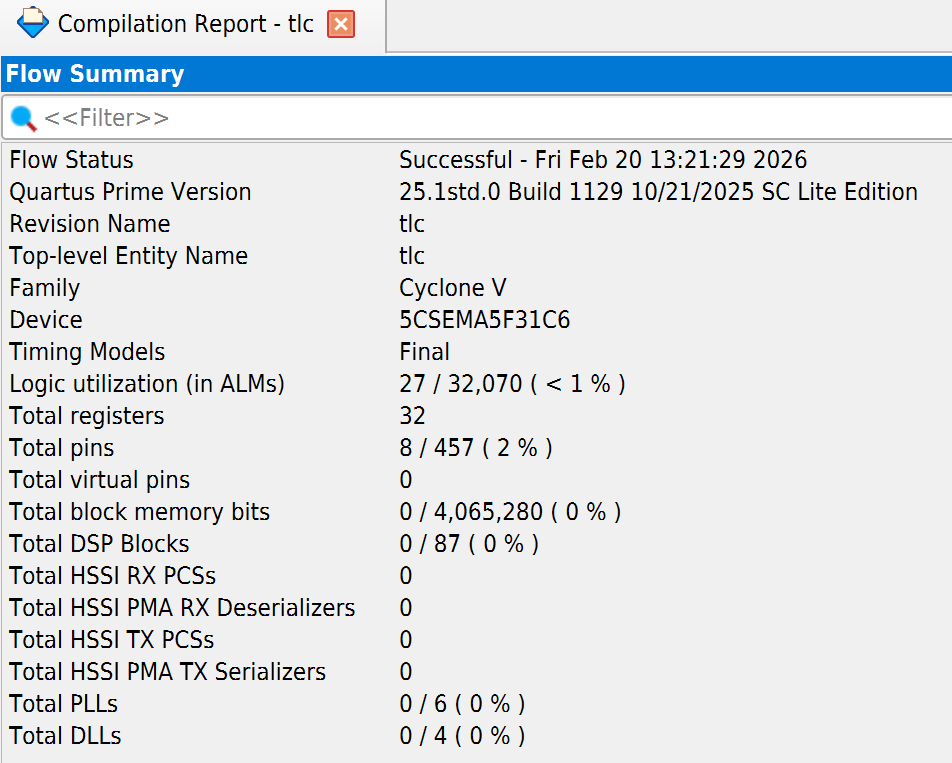
\includegraphics[width=0.5\textwidth]{images/compilation_report.png}
    \caption{Quartus Prime Compiler Flow Summary for the basic TLC design.}
    \label{fig:compilation-report}
\end{figure}

\subsection{Board Photo}
\begin{figure}[htbp]
    \centering
    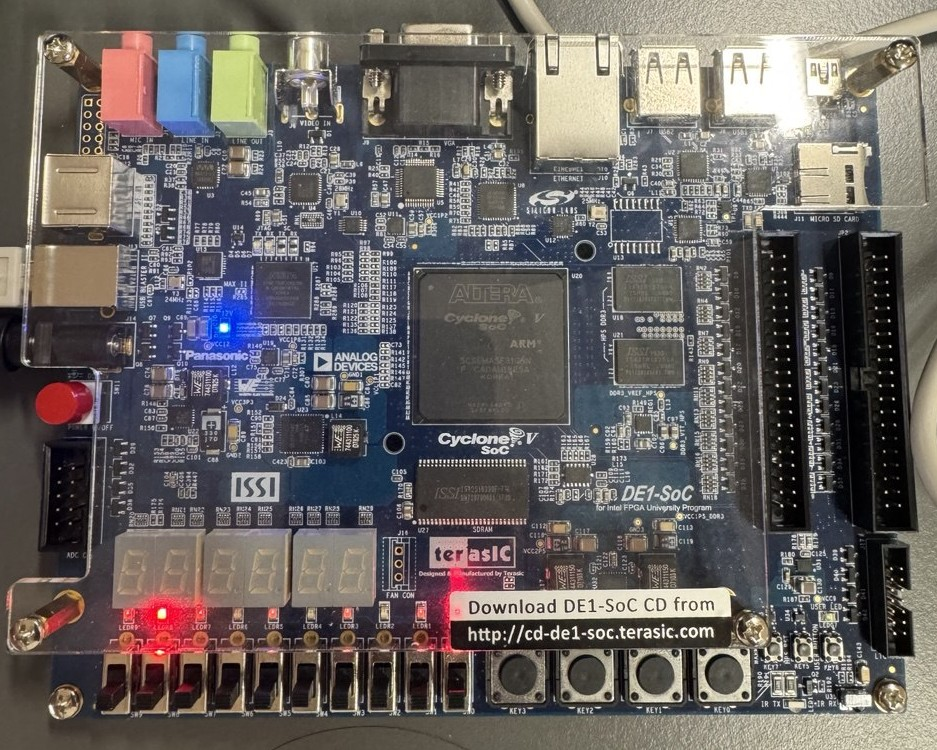
\includegraphics[width=0.5\textwidth]{images/fpga_board.jpg}
    \caption{DE1-SoC board in state \texttt{G}: LEDR8 (vehicle GREEN) and LEDR0 (pedestrian RED) are lit.}
    \label{fig:board-stateG}
\end{figure}

\subsection{Testbench}
\lstinputlisting[style=verilog, caption={Testbench for the basic TLC.}, label={lst:tb}]{tlc_tb.v}

\end{document}